% !TEX root = ../main.tex

%%%%%%%%%%%%%%%%%%%%%%%%%%%%%%%%%%%%%%%%%%%%%%%%%%%%%%%%%%%%%%%%%%%%%%%%%%%%%%%% 
%%% Background
%%%%%%%%%%%%%%%%%%%%%%%%%%%%%%%%%%%%%%%%%%%%%%%%%%%%%%%%%%%%%%%%%%%%%%%%%%%%%%%%


\chapter{Background}
This chapter is going to introduce concepts that may be unknown to the reader but central to the project. This chapter is purely theoretical, and no new information will be presented here. The subjects comprising this chapter include:
\begin{itemize}
\item An introduction to the reversible programming paradigm (Section \ref{Reverse}), as well as the language used in this project (Section \ref{Hermes}).
\item An overview of the two public-key cryptosystems that will be attempted implemented (Section \ref{Async}).
\item Some theory on Galois fields and arithmetic functions therein (Section \ref{Galois}).
\end{itemize}
The math for both RSA and Elliptic Curves is mostly based on the corresponding chapters in \cite{IntroToMath}, while Galois field theory comes from \cite{FiniteFieldArithmetic}.

%%%%%%%%%%%%%%%%%%%%%%%%%%%%%%%%%%%%%%%%%%%%%%%%%%%%%%%%%%%%%%%%%%%%%%%%%%%%%%%%
%%% Section on reversible programming. 
%%%%%%%%%%%%%%%%%%%%%%%%%%%%%%%%%%%%%%%%%%%%%%%%%%%%%%%%%%%%%%%%%%%%%%%%%%%%%%%%
% !TEX root = ../main.tex

\section{Reversible computations}
\label{Reverse}
Reversible programming is an unknown concept to many programmers, as popular programming languages are inherently irreversible. This is because the machines which are available nowadays, are built with irreversible circuits. Consider an \texttt{OR} gate in a computer. If the output from the gate is a high voltage (representing the value 1), there is some information lost, about the input for the gate. As a high voltage can be the result of either two high voltages or two different combinations of high/low voltage there is no way to reverse the operation. The same can be said for \texttt{AND} gates, but with low voltage output. Not all gates are irreversible, and the \texttt{NOT} gate does not lose any information.

It is possible to implement gates that do not lose information about the input, but that usually means additional information needed in the output. One example is a Toffoli-gate\cite{Toffoli}, which takes three inputs and produces three outputs. The gate outputs the first two bits unchanged and flips the third bit if the two first were set.

\begin{gather}
\mathtt{Input}~~~~~~~~~~~\mathtt{Output}\\
\begin{tabular}{lll}
0 & 0 & 0 \\
0 & 0 & 1 \\
0 & 1 & 0 \\
0 & 1 & 1 \\
1 & 0 & 0 \\
1 & 0 & 1 \\
1 & 1 & 0 \\
1 & 1 & 1
\end{tabular}
\rightarrow
\begin{tabular}{lll}
0 & 0 & 0 \\
0 & 0 & 1 \\
0 & 1 & 0 \\
0 & 1 & 1 \\
1 & 0 & 0 \\
1 & 0 & 1 \\
1 & 1 & 1 \\
1 & 1 & 0
\end{tabular}
\end{gather}
Simpler reversible gates are possible, but the Toffoli-gate is universal.

Reversible programming languages can still be implemented to run on machines with an irreversible architecture. As the architecture does not allow for running backward, this means compiling the code as two programs: the forward program and the reverse program. Restrictions when writing reversible programs will be language-dependent, but there will always be some restrictions on the way programs are written.
\subsection{A brief example of a reversible addition}
To demonstrate how reversible procedures can be achieved without fully reversible circuits, consider a simple integer addition. This is an irreversible operation, as it is not possible to derive the operands, given only the result of the addition. To make such an operation reversible there are a few different approaches that can be taken.

One way to make this operation reversible would be to extend the output of the operation in some way. The simplest solution would be to just include one operand in the output, as well as the sum of the two operands. This is a perfectly fine reversible operation, but it is not the only way to achieve reversible addition.

Alternatively, the output can be changed to include both the sum and the difference between the two operands. This means a somewhat altered operation, and some might argue a more versatile operation, but it does also mean a trade-off in performance, as it now needs to perform both the addition and the subtraction.

Finally, reversible addition can also be achieved by using updates. This means that addition is no longer a binary operation, but rather something that can be done to a variable. The update \texttt{+=} should be fairly familiar to the reader, and can certainly be used as a reversible addition. To make it truly reversible, however, certain constraints must be enforced. To avoid the possibility of irreversibly updating variables, the variable to be updated is commonly not allowed on the right-hand side of the update. If it was allowed to appear in the expression on the right-hand side, it would be possible to make updates such as \texttt{x += (-x)} which is indeed an irreversible update.

So achieving reversibility can come at the cost of either verbosity or complexity/restrictiveness.
\subsection{Why reversibility?}
\label{why}
The main concern comes from energy usage. The German physicist Rolf Landauer proposed a principle (Landauer's principle\cite{Landauer}) that places a lower theoretical bound on energy dissipation when performing irreversible computations\footnote{The principle states that any irreversible computation will dissipate a minimum amount of energy $Q \geq ln2 k_{b}T$.}. Although the amount is tiny, computers are getting within some orders of magnitude of the limit, and so this might become a real problem if Moore's law\footnote{The principle that the number of transistors in a dense integrated circuit will double every two years.} continues to hold. With this lower bound on energy consumption, there will be a real issue with heat in such circuits\cite{KUreverse}.

Another incentive for reversible programming is attempting to make some programming tasks easier. Since certain programming disciplines are reversible by nature, it should be easier to implement a reversible algorithm, that can then be run backwards for the inverse. 
\section{Hermes}
\label{Hermes}
The reversible language for this project is Hermes\cite{PSI19}. Hermes is inspired by the reversible language Janus and has a very C-like syntax. The language is designed specifically with encryption in mind, and apart from having several features that are commonly used in cryptography (such as rotations), the language is also designed to eliminate side-channel attacks on the encryption. The syntax for Hermes can be seen in Figure \ref{Hermes-syntax}.
\begin{figure}[h!] 
\centering 
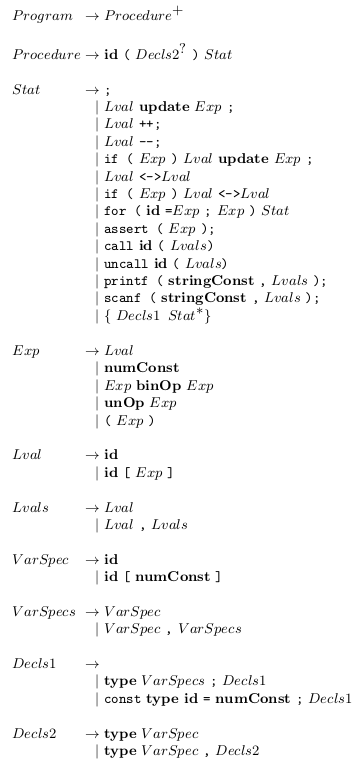
\includegraphics[width=0.6\linewidth]{figures/syntax}
\caption{Syntax of Hermes.}
\label{Hermes-syntax}
\end{figure}
\subsection{Side-channels in Hermes}
One type of side-channel that can be problematic in cryptography is residual information left in memory after running the program. Such information might contain keys, partially or in their entirety, or pieces of the plaintext that was encrypted. This is problematic but is avoided in Hermes by having all variables returned to zero before executing the program. This zeroing of variables serves another purpose, apart from avoiding data-based side-channels, as it also helps with reversibility. Consider a program that finishes by subtracting something from a variable to zero it. When running in reverse, the inverse of that operation would be to add that same value to the variable. 

%%%%%%%%%%%%%%%%%%%%% Check lige med michael om det er relativt nyt at angribe ved at kigge på timing. 
Another type of side-channel attack is timing-based side-channel attacks. Several precautions have been taken with Hermes to avoid such attacks, including:
\begin{itemize}
\item Not including time-sensitive control structures. This means that Hermes does not support \texttt{while}-loops, and that \texttt{for}-loops are restricted to iterating over a loop-local variable, which may only be updated with unconditional constant updates. 
\item Conditional updates are always evaluated. That is to say, that even if a condition is not true, the right-hand side of the update is still evaluated, to avoid value-dependent timings.
\item Logical operators like \texttt{\&\&}, \texttt{||} and \texttt{!} are not included in Hermes, only the binary equivalents.
\end{itemize}
There are more restrictions that the programmer needs to abide by when coding programs in Hermes. For a more comprehensive insight into the restrictions of Hermes, refer to \cite{PSI19}.

\subsection{Values in Hermes}
In Hermes there are three basic values to work with:
\begin{itemize}
\item Constants: These are initiated with a value and cannot be modified, which also means that they need not be zeroed before execution.
\item Variables: These may be integers, signed or unsigned, of either 8, 16, 32, or 64 bits. Variables must be zeroed before execution. 
\item Arrays: Elements must be of the same type as variables, and the size of arrays must be specified at declaration. Arrays, like variables, must be zeroed before exiting their scope. 
\end{itemize}
When working with arrays or variables, the values are never overwritten in fashions akin to:
\begin{verbatim}
u8 x = 3;
x = 4;
\end{verbatim}
Overwriting values like that is not reversible, so rather than overwriting, values are updated or swapped:
\begin{verbatim}
u8 x, y; // Values are initially zero.
x += 3;  // Assigning 3 to x by addition. 
y += 4;  // Assigning 4 to y by addition.
x <-> y; // Swapping the values in x and y. 
x -= 4;  // Reverting x to zero by subtraction. 
y -= 3;  // Reverting y to zero by subtraction.
\end{verbatim}
Here making sure to return the variables to zero before executing. 

%%%%%%%%%%%%%%%%%%%%%%%%%%%%%%%%%%%%%%%%%%%%%%%%%%%%%%%%%%%%%%%%%%%%%%%%%%%%%%%%%%%%%%%%%%%%%%%%%%%
%%%%%%%%%%%%%%%% Her er jeg nået til %%%%%%%%%%%%%%%%%%%%%%%%%%%%%%%%%%%%%%%%%%%%%%%%%%%%%%%%%%%%%%
%%%%%%%%%%%%%%%%%%%%%%%%%%%%%%%%%%%%%%%%%%%%%%%%%%%%%%%%%%%%%%%%%%%%%%%%%%%%%%%%%%%%%%%%%%%%%%%%%%%
%%%%%%%%%%%%%% Alt herunder er lidt bare gentagelser, så jeg har bare fjernet det. Vi mangler ikke ligefrem materiale. 

%Hermes is a reversible programming language specifically designed for encryption. Built with an offset in the reversible
%language Janus, Hermes has a C-like syntax.

% Should this be mentioned? I'm guessing it is mentioned elsewhere.
%The reversible manner implemented in Hermes makes it an adequate candidate to do so, due to the ability of decryption which be performed by running the encryption backwards.

% The reversible manner (get more in-depth)
%The original value of a variable is never overwritten. Alternatively, the value is either swapped to another temporary variable or updated reversibly.


%Importantance of talking about the semantic of Hermes this way?
%Values used in Hermes are either variables or one-dimensional arrays with elements representing signed and unsigned 32 or 64-bit two’s complement numbers

\subsection{Compiling Hermes}
\label{HC}
The original version of Hermes has had a compiler build for it. The compiler is built with Moscow ML\footnote{http://www.itu.dk/~sestoft/mosml.html}, so an installation of this is needed to build the compiler.

The source code for the compiler is included in the \texttt{src.zip} folder, along with a \texttt{Makefile} for building the compiler.

Provided a machine with Moscow ML installed, simply run the \texttt{Makefile} in the \texttt{Compiler} directory (not to confuse with the \texttt{Makefile} to compile the solution):
\begin{lstlisting}[language=C]
  $ make
\end{lstlisting}%$
This should create a \texttt{bin} folder, containing the compiler. 

Credit for the compiler goes to Malte Sølveste Velin and Sebastian Posselt \cite{Compiler}.
\subsection{Cryptography in a reversible manner}
\label{reverseCrypt}
% Nothing new here. Present some previous work on Hermes, and explain why cryptography has a particularly neat nature when it comes to reversibility. Asymmetric cryptography to come later.
Cryptography is, by nature, a reversible process. Text is obscured by encryption and then revealed again by decryption. Symmetric encryption embodies the very essence of reversibility, as decryption is exactly the inverse of encryption (hence symmetric). Extensive work has been done on symmetric encryption in Hermes. As an example, here is included the Tiny Encryption Algorithm (TEA)\cite{TEA} implementation in Hermes, presented in \cite{PSI19}, as well as the \texttt{C}-code from the Wikipedia page for TEA\cite{TEA}:
\begin{figure}[!h]\small
\begin{verbatim}
encrypt (u32 v[2], u32 k[4])
{
  u32 v0, v1, sum, k0, k1, k2, k3;
  const u32 delta = 0x9E3779B9;                   /* a key schedule constant */
  v0 <-> v[0]; v1 <-> v[1];                       /* set up */
  k0 += k[0]; k1 += k[1]; k2 += k[2]; k3 += k[3]; /* cache key */
  for (i=0; 32) {                                 /* basic cycle start */
    sum += delta;
    v0 += ((v1<<4) + k0) ^ (v1 + sum) ^ ((v1>>5) + k1);
    v1 += ((v0<<4) + k2) ^ (v0 + sum) ^ ((v0>>5) + k3);
    i++;
  }                                               /* end cycle */
  k0 -= k[0]; k1 -= k[1]; k2 -= k[2]; k3 -= k[3]; /* clear locals */
  sum -= delta << 5;                     /* alternatively, sum -= 0xC6EF3720 */
  v[0] <-> v0; v[1] <-> v1;                       /* return coded values */
}
\end{verbatim} 
\caption{Example of TEA implemented reversible in Hermes \cite{PSI19}.}
\end{figure}\\
\begin{figure}[!h]\small
\begin{verbatim}
void encrypt (uint32_t v[2], uint32_t k[4]) {
   uint32_t v0=v[0], v1=v[1], sum=0, i;          /* set up */
   uint32_t delta=0x9E3779B9;                    /* a key schedule constant */
   uint32_t k0=k[0], k1=k[1], k2=k[2], k3=k[3];  /* cache key */
   for (i=0; i<32; i++) {                        /* basic cycle start */
      sum += delta;
      v0 += ((v1<<4) + k0) ^ (v1 + sum) ^ ((v1>>5) + k1);
      v1 += ((v0<<4) + k2) ^ (v0 + sum) ^ ((v0>>5) + k3);
   }                                             /* end cycle */
   v[0]=v0; v[1]=v1;
}

void decrypt (uint32_t v[2], uint32_t k[4]) {
   uint32_t v0=v[0], v1=v[1], sum=0xC6EF3720, i; /* set up; sum is 32*delta */
   uint32_t delta=0x9E3779B9;                    /* a key schedule constant */
   uint32_t k0=k[0], k1=k[1], k2=k[2], k3=k[3];  /* cache key */
   for (i=0; i<32; i++) {                        /* basic cycle start */
      v1 -= ((v0<<4) + k2) ^ (v0 + sum) ^ ((v0>>5) + k3);
      v0 -= ((v1<<4) + k0) ^ (v1 + sum) ^ ((v1>>5) + k1);
      sum -= delta;
   }                                             /* end cycle */
   v[0]=v0; v[1]=v1;
}
\end{verbatim} 
\caption{Example of TEA implemented in C \cite{PSI19}.}
\end{figure}
\\
As seen in the example, when implementing symmetric encryption algorithms in a reversible language, as opposed to a regular irreversible language, only one method is needed in place of two (one for encryption and one for decryption).

This neat property is only applicable to symmetric encryption. When implementing asymmetric cryptography, there will still be a need for two functions, as encryption and decryption are not simply each other's inverses.


%%%%%%%%%%%%%%%%%%%%%%%%%%%%%%%%%%%%%%%%%%%%%%%%%%%%%%%%%%%%%%%%%%%%%%%%%%%%%%%%
%%% Section on asymmetric cryptography. 
%%%%%%%%%%%%%%%%%%%%%%%%%%%%%%%%%%%%%%%%%%%%%%%%%%%%%%%%%%%%%%%%%%%%%%%%%%%%%%%%
% !TEX root = ../main.tex

\section{Asymmetric cryptography}
\label{Async}
Asymmetric cryptography\footnote{Often also referred to as Public-key cryptography.} is a term used to describe crypto-systems that use key pairs rather than a common shared secret - as in symmetric cryptography. The key pair consists of a private key, only known to the owner of the key pair, and a public key that is visible to the public.

Asymmetric cryptography covers more than simply encryption and decryption. Key generation can also be done asymmetrically with schemes such as the Diffie-Hellman key exchange. This sort of asymmetric cryptography will not be a focus in this paper, as encryption/decryption is the main focus.

There is, however, a third use for asymmetric cryptography, which will become interesting when all of this is done reversibly: digital signatures. With the private key being known only to the owner, anything that can be successfully decrypted with the public key can therefore only have been sent by them.
\subsection{RSA}
\label{RSA}
RSA is an asymmetric cryptosystem developed in the 1970s by Ron \textbf{R}ivest, Adi \textbf{S}hamir, and Leonard \textbf{A}dleman, and is arguably the best known and most commonly used cryptography algorithm\cite{RSA}. It implements the public/private key pair infrastructure used in asymmetric cryptography and uses integer factorization to provide security.

\subsubsection{Integer Factorization}
The algorithm makes use of the integer factorization problem which deals with the decomposition of a composite number\cite{integerfactor}. It is well known to be significantly harder to find the factor of a product, than calculating the product of two integers. The RSA algorithm, therefore, assumes that it is computationally expensive to solve the prime factorization problem given a large composite \textit{n}, such that $n=p \cdot q$ where $p\neq q$ and $p$ and $q$ are both prime\cite{RSA}. This essentially works as a one-way trap door function, which is easy to compute in one direction, but almost impossible to perform in the reverse direction. An example of this can be seen below:
$$n = p \cdot q = 44560482149 \cdot 6620830889=295027416640832300461$$


%This \textit{n} might be rather trivial to factorize for a computer, and it is therefore important to choose sufficiently large prime numbers, to generate a large enough \textit{n}. This \textit{n} will be used as the modulus for both the private and public keys as well as for key-generation. Hence the National Institute of Standards and Technology suggests a bit-length of at least 2048 to provide adequate security\cite{RecommendationForKeyManagement}. 

This value of \textit{n} might be rather trivial to factorize for a computer, and it is, therefore, important to choose sufficiently large prime numbers, to generate a large enough \textit{n}. This \textit{n} will be used as the modulus for both the private and public keys as well as key-generation in the cryptographic stage of the algorithm. Hence the National Institute of Standards and Technology suggests a bit-length of at least 2048 to provide adequate security \cite{RecommendationForKeyManagement}. 

% https://nvlpubs.nist.gov/nistpubs/SpecialPublications/NIST.SP.800-57Pt3r1.pdf

% n used in key generation? Er det egentlig det? Det er jo faktisk phi af n som man bruger til at generere krypterings exponenten



% the fundamental theorem of arithmetic, every positive integer has a unique prime factorization.

%%%%%%%%%%%%%%%%%%%%%%%%%%%%%%%%%%%%%%%%%%%%%%%%%%%%%%%%%%%%%%%%%%%%%%%%%%%%
%%% Danny freestyler lige lidt, det er ikke nødvendigvis noget der skal med i rapporten.
\subsubsection*{Modular exponentiation}
The goal of this project is only encryption/decryption (no key generation), which in RSA essentially boils down to modular exponentiation. A promising method for implementing modular exponentiation (specifically considering Hermes), is a left-to-right binary method. The reason this method is more appealing than others is the looping over binary representations. Since looping is rather restricted in Hermes, this is a good method for looping, while staying within the boundaries of Hermes. A more in-depth look at this method will be provided in Chapter \ref{OurRSA}. 

%Recall from section \ref{Hermes}, that Hermes is restricted in several ways, to eliminate time-based side-channel attacks. These restrictions become somewhat troublesome when attempting to implement exponentiation, as execution time for exponentiation is very much dependent on the exponent. As RSA implementations are, omitting key generation, simply modular exponentiation, this is a bit of a bump in the road. To get around this, it is necessary to investigate different approaches to modular exponentiation.
%%% Talk a bit about Exponentiation by squaring and left-to-right binary method. More about the one that turns out to work, if any! 
%%%%%%%%%%%%%%%%%%%%%%%%%%%%%%%%%%%%%%%%%%%%%%%%%%%%%%%%%%%%%%%%%%%%%%%%%%%%

%>>>>>>>>>>>>>>>>Head
%\subsubsection{Public key cryptosystem}
%The private key \textit{d} and a public key \textit{e} are defined has two keys used to decrypt and encrypt messages when communicating. The couple ($N,e$) constitutes the public key, where $n=p \cdot q$ is the modulus and $e$ the encryption exponent. However, \textit{e} cannot be picked randomly and must therefore obey the following properties:
%=================
\subsubsection{RSA discrete logarithm problem}
Commonly referred to as the RSA problem\cite{RSAProblem}, it refers to the infeasibility of computing $m$ in $C=m^e ~ (mod ~ n)$ given the RSA public key $(n,e)$ and the ciphertext $C$, for a sufficiently large $n$. Given that it is trivial to compute in one direction, and practically impossible to do in reserve, is known as a one-way trapdoor function. This is closely related to the integer factorization problem and is together the basis of security for the RSA encryption scheme . 


\subsubsection{Public/Private key cryptosystem}
The private key \textit{(d,n)} and a public key \textit{(e,n)} are used to decrypt and encrypt respectively. The pair ($N,e$) constitutes the public key, where $n=p \cdot q$ is the modulus and $e$ the encryption exponent. However, \textit{e} cannot be picked randomly and must therefore obey the following properties: 
\[e=\begin{Bmatrix}
1 < e < \phi (n)   \\
e \bot N, \phi (n)
\end{Bmatrix}
\]
Where $\phi (N) = (p-1)(q-1)$.

When encrypting a message using RSA, a message \textit{m} must first be converted to integers using a binary translation.% To perform the encryption step, both parties must first exchange their public keys (\textit{N,e}).
The sender of the message can now apply the receiver's public key to encrypt the message \textit{m} into ciphertext \textit{c} using the following formula:

$$c \equiv m^{e}(mod ~ N)$$

After having performed this step, the sender is now able to communicate the ciphertext \textit{c} to the correspondent. Recovering the original message from \textit{c} requires the use of the private key $(N,d)$.% The decryption exponent \textit{d} is derived by taking modular multiplicative inverse of $e ~ (mod ~ \phi (N))$, which is straightforward since information about $\phi (N) = (p-1)(q-1)$ is known to the owner of the public and private key.
The receiver of the message now recover the plaintext \textit{m} by computing:


%Reverting the ciphertext \textit{c} back into the original message $m$ requires the use of the private key $(N,d)$. The decryption exponent \textit{d} is derived by taking modular multiplicative inverse of $e ~ (mod ~ \phi (N))$, which is straightforward since information about $\phi (N) = (p-1)(q-1)$ is known to the owner of the public and private key. The receiver of the message now recover the plaintext \textit{m} by computing:

$$c^d ~(mod ~~ N)\equiv (m^e)^d ~(mod ~~ N)\equiv m^{ed} ~(mod ~~ N)\equiv m^{N \phi(N)+1} ~(mod ~~ N)\equiv M$$

\newpage

\subsection{Elliptic curve cryptography}
\label{elliptic}
Elliptic curve cryptography (ECC) is another asymmetric cryptosystem. The curve itself is a function on the form $E: ~ y^2 \equiv x^3+ax+b $ also called a Weierstrass curve, where $a$ and $b$ are the parameters of the curve\cite{elipticcurve}. The shape of the curve changes with these parameters. %%%%%%%
%ECC uses the same underlying principles as other public key cryptosystems of the form $g^a ~ mod ~n$, where \textit{g} is the generator, \textit{a} is the secret exponent and \textit{n} is the modulus $n \in \mathbb{P}$. However, in ECC this is done over an elliptic curve structure.
\begin{figure}[H]
    \centering
    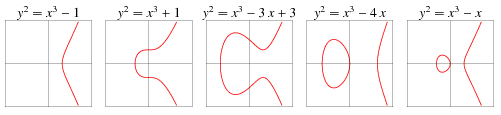
\includegraphics[width=1.0\textwidth]{figures/elliptic-curve-example}
    \caption{Example shapes of elliptic curves given different parameters $a,b$ in the form  $E: ~ y^2 \equiv x^3+ax+b $}
\end{figure}
\noindent This structure can be defined by the equation:
$$\{(x,y) \in \mathbb{R}^{2} ~ | ~ y^2 \equiv x^3 +ax +b, 4a^3 + 27b^2 \not\equiv 0 \} \cup \{0\}$$
where $4a^3+27b^2 \neq 0$ to avoid singular points.

The geometry of elliptic curves allows for adding points together. This point-addition is not the same as regular arithmetic addition, but shares some properties with it, hence the name. 
\subsubsection{Elliptic Curve Point-Addition}
\label{ECPA}
Adition on an elliptic curve is not an actual arithmetic operation, but rather a geometrical one. It is done by drawing a line through the two points, which will intersect the curve at a third point $R'$. Reflecting this new point $R'$ on the x-axis results in yet another point on the curve, called $R$.

$$P \oplus Q = R$$

For this operation to properly inherit the properties of arithmetic addition, an additive identity is necessary. This is what is referred to as the point-at-infinity, and is denoted $\mathcal{O}$. This point is the result of any addition which draws a perfectly vertical line through the two points\cite{IntroToMath}. 
%\mathcal{O}

The addition law on an elliptic curve \textit{E} can now be described as:\\
\begin{figure}[H]

\textbf{Theorem 6.5}. \textit{Let E be an elliptic curve. Then the addition law on E has the following properties:}\\
(a) $~~~~~ P + \mathcal{O} = \mathcal{O} + P = P ~~~~~~~~~~~~~~~ for ~ all ~~ P \in E. ~~~~~~~~~ [\text{Identity}]$ \\
(b) $~~~~~ P + (-P) = \mathcal{O} ~~~~~~~~~~~~~~~~~~~~~~ for ~ all ~~ P \in E. ~~~~~~~~~~ [\text{Inverse}]$ \\
(c) $~~~~ (P+Q) + R = P+(Q+R) ~~~~~ for ~ all ~~ P,Q,R \in E. ~~~ [\text{Assosiative}]$ \\
(d) $~~~~~~ P + Q = Q+P ~~~~~~~~~~~~~~~~~~~~ for ~ all ~~ P,Q \in E. ~~~~~~~~ [\text{Commutative}]$ 
\caption{Theorem 6.5: Addition law on elliptic curves\cite{IntroToMath}.}
\end{figure}


Notice how the theorem refers to a negation of a point ($-P$). This negation can be understood as flipping the point over the curve, and so if $P=\{x,y\}$ then $-P=\{x,-y\}$.

\begin{figure}[H]
    \centering
    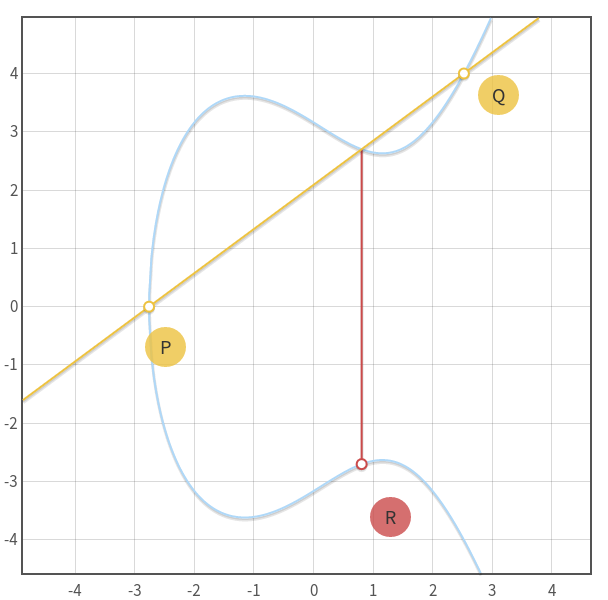
\includegraphics[width=0.7\textwidth]{figures/ECC-point-addition}
    \caption{Illustrating Point addition over the elliptic curve $y^2 = x^3 - 4x + 10$ in $\mathbb{R}$ where $P = (-2.76082, 0)$, $Q = (2.5251, 5)$ and $R = (0.80836, -2.70089)$.}
\end{figure}

\noindent The coordinates of a point $R = P\oplus Q$ are defined as:
\[R_x:= \lambda^2-P_x-Q_x\]
\[R_y:= -P_y+\lambda(P_x-R_x)\]
Where $\lambda$ is defined as:
\[\lambda := \frac{P_y-Q_y}{P_x-Q_x}\]

\subsubsection{Point-Doubling}
A special case of point addition is that in which the two points have the same coordinates: $P={x,y}=Q$. This case is referred to as point doubling and is done slightly differently than the addition of two distinct points.

To double a point, the line that is followed is the tangent at the point $P$. If $P_y \neq 0$, then this tangent line will intercept the curve at another point $R'$, and flipping the point over the $x$-axis yields the result $R$.

If, on the other hand, $P_y = 0$ then $R=2P = \mathcal{O}$, as the tangent in such a point will be vertical. 

\noindent The coordinates of the point $R=2P$ are defined similarly to simple addition:
\[R_x:= \lambda^2-2P_x\]
\[R_y:= -P_y+\lambda(P_x-R_x)\]
except for the calculations for finding $\lambda$:
\[\lambda := \frac{3*P_x^2+a}{2P_y}\]
where $a$ is $a$-coefficient from the curve.

\subsubsection{Point-Multiplication}
With a point-addition defined, repeatedly adding a point to itself is called point-multiplication (just like multiplication is defined in regular arithmetics). That is, a point $P$ multiplied by a number $n$ is defined as:
$$nP = \underbrace{P\oplus P\oplus P\oplus \ldots \oplus P}_\text{n copies}$$
This operation is the core of elliptic curve cryptography (ECC), in both key generation and encryption/decryption.

For any curve used in ECC, points for multiplication are not chosen at random. Instead a generator point $G$ is chosen for a curve, which can then be added to itself any number of times.

\subsubsection{Elliptic curve discrete logarithm problem}
Having multiplied a point $G$ by some number $n$, yielding a new number, is a process that is computationally infeasible to retrace. Given a curve $E$ and the points $G, Q \in E$, one would have to find an integer \textit{n}, if it exists, such that $Q = nG$. This is known as the “elliptic curve discrete logarithm problem” (ECDLP)\cite{elipticcurve}\cite{logarithmproblem}.
% WierStrass Form: https://crypto.stanford.edu/pbc/notes/elliptic/weier.html


\subsubsection{Elliptic Curve over Finite Fields}
Elliptic curve arithmetics over a real number plane $(x,y) \in \mathbb{R}$ is often used to exemplify the computational steps in the arithmetics. However, ECC is typically done over a predefined finite field.

When limiting the points from $\mathbb{R}$ to ${\mathbb{F}_p}$ or ${\mathbb{F}_p}^2$ the curve is then defined by:
$$\{(x,y) \in \mathbb{F}_{p} ~ | ~ y^2 \equiv x^3 +ax +b ~ (mod ~ p), 4a^3 + 27b^2 \not\equiv 0 ~ (mod ~ p) \} \cup \{0\}$$
Here $x,y$ are constant values from a finite field $\mathbb{F}_{p}$, where p is a prime number that determines the size of the field\cite{elipticcurvefinite}. Not only must coordinates be within the field, but the same goes for the coefficients of the curve: $a,b\in\mathbb{F}_p$.

Addition and multiplication are performed in the same manner, except all computations are performed $mod~p$.

This representation means that the curve no longer looks the same, as it is now a seemingly scattered group of points. There is, however, still symmetry in the points, as the curve has, in a sense, simply been shifted up above the $x$-axis. 
%The point $P$ specifies a predetermined base point also called the generator point $G=(x_P, y_P)$ on the curve and \textit{n} is a prime of the order of $P$ which initially determines the maximum value that can be turned into a private key.

\begin{figure}[H]
    \centering
    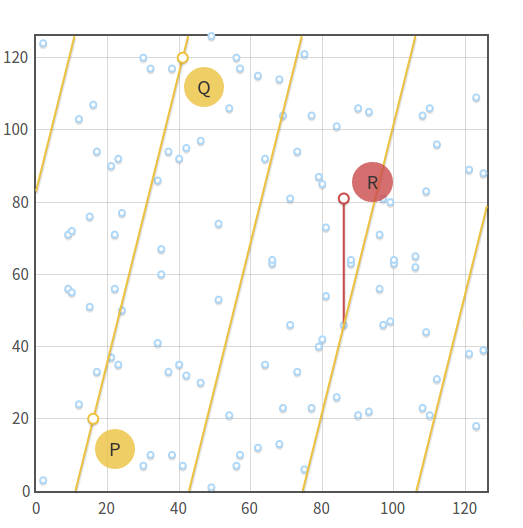
\includegraphics[width=0.6\textwidth]{figures/ECC-finite-field}
    \caption{Example of point addition over the curve $y^2 = x^3-x+3$ in $\mathbb{F}_{127}$ with $P = (16, 20)$, $Q = (41, 120)$ and $R = (86, 81)$}
\end{figure}

Not all curves are pleasant to work with, and proving properties about them is a difficult process. NIST has published a collection of suggested curves over a variety of Finite Fields (both prime fields, as described here, but also extension fields, more on that in Section \ref{Galois}).
\subsubsection{Elliptic Curve Integrated Encryption Scheme (ECIES)}
For an elliptic curve $E$ on the form $y^2=x^3+ax+b$ over a prime field $\mathbb{F}_p$, the encryption is rather elegant\footnote{https://asecuritysite.com/encryption/ecc3}. With some generator point, $G$, for the curve, a person (say Alice, the usual suspect) can produce a public/private key-pair by choosing a random number $d$ and multiplying that with the generator point $G$: $dG=Q$. The new point $Q$ is the public key, and the random number $d$ is the private key. 

When a sender (say Bob, Alice's ages-old friend) wants to encrypt a message for Alice, he does the following:
\begin{enumerate}
\item Chooses a random number $r$.
\item Generates 2 new points: $S=rQ$ and $R=rG$.
\item Derives a key from the point $S$ using an arbitrary Key Derivation Function (KDF) and symmetrically encrypts his message using that key.
\item Sends his encrypted message, as well as the point $R$ to Alice.
\end{enumerate}
Alice can now decrypt the message by:
\begin{enumerate}
\item Computing the point $S$ by multiplying the point $R$ sent to her by Bob with her private key $d$.
\item Deriving a key from the point $S$ using the same Key Derivation Function (KDF).
\item Symmetrically decrypting the message with the key.
\end{enumerate}
To see why this works, consider:
\[S=rQ=rdG=drG=dR\]
This holds due to the properties of point-addition described in Section \ref{ECPA}. 
\newpage

%%%% UNUSED/REWRITTEN STUFF %%%%

%================================================================================
%\noindent This point addition is now repeated by drawing a line through \textit{P} and \textit{R'}, thus intersection with a new point \textit{Q} on the curve. Again, we find the inverse of this point and repeat the same operation. 


%However, instead of adding two arbitrary points, we use a specific base point \textit{P} on the curve which will be added together.


%The same operation is used to add and reflect the point across the x-axis. however now we just continuously add \textit{P} together, thus computing $nP$. For a point \textit{P} on the elliptic curve and a non-negative scalar \textit{n}, we now define $nP$ to be:
%$$nP = \underbrace{P+P+P+ \ldots + P}_\text{n copies}$$

%<<<<<<< HEAD
%Performing this operation \textit{n} times will yield a final point $Q = nP$. These elements will be used as keys in the cryptosystem, due to the infeasibility of findiæng \textit{n} even though you have the starting point \textit{P} and some ending point \textit{Q}. ECC, therefore, exploits the difficulty of computing the discrete logarithm of a random elliptic curve element for a publicly known base point, or the “elliptic curve discrete logarithm problem” (ECDLP)\cite{elipticcurve}. 
%=======
%This repeated addition is called point multiplication. Performing this operation \textit{n} times will yield a final point $Q = nP$. These elements will be used as keys in the cryptosystem, due to the infeasibility of finding \textit{n} even though you have the starting point \textit{P} and some ending point \textit{Q}. ECC, therefore, exploits the difficulty of computing the discrete logarithm of a random elliptic curve element for a publicly known base point, or the “elliptic curve discrete logarithm problem” (ECDLP)\cite{elipticcurve}. 


%\subsubsection{Point at infinity}
%Recall from theorem 6.5 in \ref{mylabel} how the identity element of an elliptic curve is defined for elliptic curve addition:
%\begin{align*}
%\mathcal{O} + P = P \\
%P + (-P) = \mathcal{O} 
%\end{align*}

%\noindent Both the identity and inverse law requires a point $\mathcal{O}$ to exist to be true. This point on the curve is defined as the identity element also called point at infinity and lies on all vertical lines and can be written as (0,0). 

%\textbf{Skal nedstående med?}\\
%Showing that for any point $P$ there exist an inverse is now a trivial task due to our point at infinity as we know that when reflecting the point at infinity $-\mathcal{O} = \mathcal{O}$, it yields the same point at infinity showing that an inversion is the same \textit{x-coordinate} but with an inverse \textit{y-coordinate} consequently showing that $P + (-P) = \mathcal{O}$\\
%\textbf{slutter her}
%\begin{figure}[H]
%    \centering
%    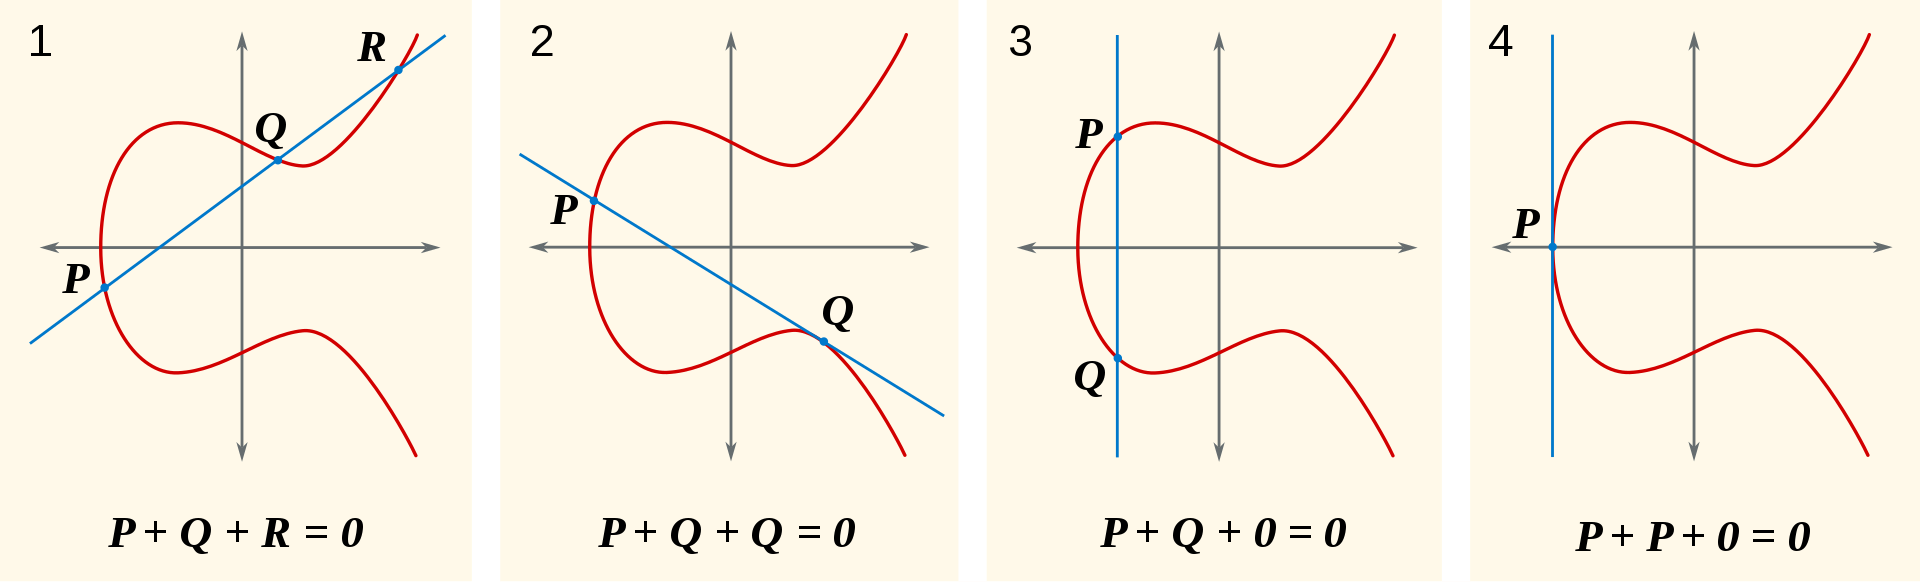
\includegraphics[width=1.0\linewidth]{figures/pointofinfinity}
%    \caption{Elliptic curve point operations: Addition (shown in facet 1), doubling (facets 2 and 4) and negation (facet 3).}
%    \label{fig:pointofinfinity}
%\end{figure}
%The ability to sum two points on the curve in simple Weierstrass form, which are each others' inverses, is not possible without the existence of point at infinity, because it would require the diversion of zero, which is not an allowed operation. This also means that the slope cannot be calculated because $P_x = Q_x$ as can be seen in facet 3 and 4 in figure \ref{fig:pointofinfinity}. Similar problem arises when trying to double a point $P_x = 0$. Hence the point at infinity is there to fill these gaps in the elliptic curve addition and acts as a neutral element (zero)\cite{IntroToMath}.
%>>>>>>> 893ba619fd33b3d23df071caa73202bb7cdfce33



% Question: Should the section below be either split up, rewritten, or placed elsewhere?









%%%%%%%%%%%%%%%%%%%%%%%%%%%%%%%%%%%%%%%%%%%%%%%%%%%%%%%%%%%%%%%%%%%%%%%%%%%%%%%%
%%% Section on finite field arithmetics.  
%%%%%%%%%%%%%%%%%%%%%%%%%%%%%%%%%%%%%%%%%%%%%%%%%%%%%%%%%%%%%%%%%%%%%%%%%%%%%%%%
\section{Finite fields}
\label{Galois} 
Finite fields, synonymously Galois fields after french mathematician Évariste Galois (25th October 1811 - 31st May 1832 (shot dead in a duel)\footnote{https://en.wikipedia.org/wiki/\%C3\%89variste\_Galois}), are sets with a finite number of elements. Apart from having a finite number of elements, such a set must be closed under addition, subtraction, multiplication, and division.

Apart from the need for finite fields in elliptic curve cryptography, the motivation for investigating finite fields comes from the irreversible nature of prime factorization. To be able to make RSA reversible, finite fields will hopefully make that task possible. 
\subsection{Field theory} %%Overvej en anden headline til denne section, e.g. "composition of finite fields" eller noget. 
A Galois field cannot have any number of elements. For the set to be able to satisfy the above-mentioned requirements (closed under certain operations), the number of elements in the set must be either prime or a power of a prime. The simplest fields to work with, are those with $p$ elements, where $p$ is prime. These fields, aptly named Prime Fields, contain the integer numbers $\mathbb{F}_p=\{0,1,2,..,p-1\}$\footnote{The notation $\mathbb{F}_p$ is shorthand for the Field with $p$ elements.}.

A finite field can, as previously mentioned, also have a number of elements that is equal to the power of a prime. More generally, Galois Fields must have $p^m$ number of elements, where $p$ must be prime, and $m$ must be a positive integer. By this definition, Prime Fields are simply Galois Fields with $p^1$ elements. A Galois Field with $m>1$ is called an Extension Field, and consist of more complicated elements. To be able to keep the set closed under addition and multiplication, the elements of the set must be polynomials rather than integers. The polynomials in an Extension Field are on the form:
\[c_1x^{m-1}+..+c_{m-1}x+c_{m}\]
where the constants $c_{i}$ with $0<i\leq m$ are integers, such that $0\leq c_{i}< p$. That is, the polynomials will be of $m-1^{th}$ degree, and the coefficients can have values ranging from $0$ to $p-1$. Other variations of extension fields exist, where the numbers are not strictly represented as polynomials, but due to the neat representation presented next, this paper will stick to polynomials for the elements of the fields.\\

A particularly interesting family of finite fields, especially in the world of computer science, are those where $p=2$. Such fields are particularly nice to encode, as the polynomials can be represented as bit-sequences. That is, a polynomial of degree 7 in $\mathtt{mod}2$, can be represented with a byte, where each bit corresponds to a nomial:
\[x^7+x^6+x^5+x^4+x^3+x^2+x+1:=11111111\]
As this is also an unsigned integer representation, it is possible to do finite field computations using integers, if working in a finite field of characteristic 2. These computations are, however, somewhat different from regular integer arithmetics, so some considerations need to be taken.

\subsection{Finite field arithmetics}
Computations in finite fields depend on the field in which they are performed. The simplest fields to do arithmetics in are prime fields. In prime fields, arithmetic operations are simply performed modulo $p$, where $p$ is the number of elements in the field. To demonstrate this, consider the finite field with 7 elements $\mathbb{F}_7=\{0,1,2,3,4,5,6\}$. This is clearly a prime field, and so arithmetics should be simple to perform. With 7 elements in the field, the computations must be performed $\mathtt{mod}7$. Any arithmetic operation that lands within the field, will remain the same, as the modulo will leave it unchanged:
\[1+2=3 ~ \mathtt{mod} ~ 7=3\]
\[4+2=6 ~ \mathtt{mod} ~ 7=6\]
\[5+2=7 ~ \mathtt{mod} ~ 7=0\]
\[2*3=6 ~ \mathtt{mod} ~ 7=6\]
\[2*4=8 ~ \mathtt{mod} ~ 7=1\]
The last product demonstrates how $2$ and $4$ are each others multiplicative inverse in the finite field $\mathbb{F}_7=\{0,1,2,3,4,5,6\}$.\\

\noindent When doing arithmetics in extension fields, there are some obvious differences, as the elements of such fields are polynomials, rather than integer numbers. Some arithmetics are, however, still fairly simple to perform. Addition and subtraction are done with regular polynomial addition/subtraction, but modulo the characteristic of the field. That is, polynomials are added/subtracted term-by-term modulo $p$. As a small example, consider the field:
\[\mathbb{F}_9=\mathbb{F}_{3^2}=\begin{Bmatrix}
0 & x   & 2x   \\
1 & x+1 & 2x+1 \\
2 & x+2 & 2x+2
\end{Bmatrix}
\]
Some simple arithmetic operations could be:
\[1+2=3 ~ \mathtt{mod} ~ 3=0\]
\[(1)+(x)=((0+1) ~ \mathtt{mod} ~ 3)x+((0+1) ~ \mathtt{mod} ~ 3)=x+1\]
\[(2x+1)+(x+2)=((2+1) ~ \mathtt{mod} ~ 3)x+((1+2) ~ \mathtt{mod} ~ 3)=0\]
Apart from the fact that the operands are polynomials, this sort of arithmetics are fairly straight forward. Unfortunately, multiplication becomes a bit more intricate. The method for addition presents several issues. First of all, multiplication modulo the characteristic of the field is ambiguous. To see this, simply consider:
\[(1*1) ~ \mathtt{mod} ~ 3=1=4 ~ \mathtt{mod} ~ 3=(2*2) ~ \mathtt{mod} ~ 3\]
Secondly, multiplying polynomials can result in a polynomial of a higher degree, even if the nominal are modulo the characteristic of the field:
\[((x+1)(2x+2)) ~ \mathtt{mod} ~ 3=2x^2+x+2\]
But this is not an element in the field, and so the field is not closed under multiplication this way. To get around these issues, multiplication needs to be done modulo an irreducible polynomial of degree $m$ for a field $\mathbb{F}_{p^m}$. This polynomial only needs to be irreducible over the field, so, simply speaking, it is a polynomial that cannot be represented as a product of two elements of the field, and that has coefficients that belong to the field. Such a polynomial always exists, and there is not necessarily only one such polynomial for a field. Therefore, it is necessary to include the irreducible polynomial in the definition of the field, as a different polynomial will result in a different field.

When a polynomial has been selected, multiplication is now done modulo this polynomial. That is, a product is found by multiplying the two operands, and then finding the remainder after long division of that product with the irreducible polynomial. To demonstrate this, the example field above can be defined with the irreducible polynomial $x^2+1$. As mentioned above, this polynomial is not uniquely irreducible in $\mathbb{F}_9$, but there are, in fact, 2 other polynomials that could be used instead: $x^2+x+2$ or $x^2+2x+2$. There exist algebraic methods for finding such irreducible polynomials\cite{findingIrreducible}, but this is outside the area of interest for this paper.

Defining the field with the polynomial $x^2+1$ can be written using the notation $\mathbb{F}_9[x]/x^2+1$.

With the polynomial determined, multiplication can now be done modulo $x^2+1$. While performing the multiplication and long division, all intermediate calculations are done modulo the characteristic of the field. To demonstrate, here is shown the computations of $(2x+2)(x+1)$:
\[(2x+2)(x+1) ~ \mathtt{mod} ~ (x^2+1)\]
\[=2x^2+x+2 ~ \mathtt{mod} ~ (x^2+1)\]
Now simply do long division, to find the remainder:\\
\begin{center}
\setstackgap{S}{1.5pt}
\stackMath\def\stackalignment{r}
\(
\stackunder{%
  x^2+1 \stackon[1pt]{\showdiv{2x^2+x+2}}{2}%
}{%
\Shortstack[l]{{\underline{2x^2\ph{+~x}+2}} \ph{2x^2+}x\ph{+2}}%
}
\)
\end{center}
And so the product of $2x+2$ and $x+1$ in $GF(3)[x]/x^2+1$ is $x$, which is indeed within the field.
\subsubsection{Arithmetics in characteristic 2 finite fields}
As mentioned at the beginning of this section, the extension fields with characteristic 2, that is $\mathbb{F}_{2^m}$, can be very neatly represented using bit-sequences. Furthermore, the arithmetics in such fields are also very pleasant to implement on a machine, as bit-wise operations can be used instead of needing to implement/use complicated libraries for polynomial arithmetics. Consider the most basic operations: addition and subtraction. In a field with characteristic 2, these operations become simpler, as adding or subtracting  $1\texttt{mod}2$ yields the same result.
\\
\begin{table}[!h]
\begin{center}
\begin{tabular}{|l|l|l|}
\hline
+/- & 0 & 1 \\ \hline
0   & 0 & 1 \\ \hline
1   & 1 & 0 \\ \hline
\end{tabular}
\end{center}
\end{table}
Note that this is the same table as that of the \texttt{XOR} (exclusive-or) operation, and so a simple polynomial addition/subtraction in a field with characteristic 2 can be done using \texttt{XOR}.

In a similar way, it is possible to implement polynomial long division using a combination of \texttt{XOR} (inplace of subtraction) and shifting. An example of a modular operation\cite{finiteFieldArithmetics} using such a method can be seen in Figure \ref{longmod}.
\begin{figure}[!h]\small
\begin{verbatim} 
          11111101111110 (mod) 100011011
         ^100011011     
          --------------
          01110000011110
          ^100011011    
           -------------
           0110110101110
           ^100011011   
            ------------
            010101110110
            ^100011011  
             -----------
             00100011010
              ^100011011
               ---------  
               000000001
\end{verbatim}
\caption{Polynomial modulo using binary operations.} 
\label{longmod}
\end{figure}


With this in mind, arithmetic operations in characteristic 2 finite fields can then be implemented as relatively simple methods, using primarily binary operations. An example can be seen in Figure \ref{finitearithmetics}. This implementation is from the Wikipedia page for finite field arithmetics\cite{finiteFieldArithmetics}, except comments have been removed to fit the page. 
\begin{figure}\small
\begin{verbatim}
uint8_t gadd(uint8_t a, uint8_t b) {
    return a ^ b;
}

uint8_t gmul(uint8_t a, uint8_t b) {
    uint8_t p = 0;
    while (a && b) {
        if (b & 1) 
            p ^= a; 

        if (a & 0x80) 
            a = (a << 1) ^ 0x11b; 
        else
            a <<= 1; 
        b >>= 1; 
    }
    return p;
}
\end{verbatim}
\caption{\texttt{C} implementation of finite field arithmetics in $\mathbb{F}_{2^8}$.}
\label{finitearithmetics}
\end{figure}